\documentclass[11pt]{article}

% ===================== PACKAGES =====================
\usepackage[margin=1in]{geometry}
\usepackage{amsmath, amssymb, amsthm}
\usepackage{graphicx}
\usepackage{tikz}
\usetikzlibrary{shapes.geometric, arrows.meta, positioning, fit, backgrounds}
\usepackage{hyperref}
\usepackage{booktabs}
\usepackage{caption}
\usepackage{algorithm}
\usepackage{algpseudocode}
\usepackage{times}
\usepackage[numbers]{natbib}

\title{\textbf{Agentic AI for Cost-Aware Hyperparameter Optimization: \\ An LLM-Driven Early-Stopping Framework}}
\author{Your Name(s) \\ Department of Computer Science and Engineering \\ VIT-AP University}
\date{}

\begin{document}

\maketitle

% ===================== ABSTRACT =====================
\begin{abstract}
Hyperparameter optimization (HPO) for deep learning models is computationally expensive, and a substantial fraction of this expense is avoidable: most trials evaluated during a search are, by design, suboptimal, yet each still incurs the full cost of training on cloud infrastructure. Existing HPO frameworks, including Tree-structured Parzen Estimator (TPE) methods and multi-fidelity approaches such as Hyperband, optimize primarily for model accuracy and reduce cost only as an incidental effect of their search strategy, without treating monetary cost as an explicit decision variable. This paper proposes an agentic approach to cost-aware hyperparameter optimization, in which a large language model (LLM) functions as an autonomous decision-making agent responsible for early-stopping decisions within the HPO loop. After each training epoch, the agent is provided with the trial's current accuracy, its loss trend, its standing relative to the best trial observed so far, the cost incurred to that point, and the remaining experimental budget. Based on this context, the agent decides whether to continue, extend, or terminate the trial, and produces a natural-language justification for its decision. We evaluate this approach on a ResNet18/CIFAR-10 image classification task, comparing agent-guided search against a random-search baseline without early stopping, using simulated cost derived from measured training time and published cloud GPU pricing. Unlike prior cost-aware HPO methods, which rely on statistical cost models or separately trained classifiers, our approach grounds termination decisions in interpretable LLM reasoning, offering a lightweight and auditable method for reducing hyperparameter search costs in deep learning workflows.

\vspace{0.5em}
\noindent\textbf{Keywords:} Agentic AI, Hyperparameter Optimization, Cost-Aware Machine Learning, Large Language Models, Early Stopping, Green AI
\end{abstract}

% =====================================================
\section{Introduction}
\label{sec:intro}

\subsection{Background and Motivation}

Deep learning models rely heavily on hyperparameter tuning: settings such as learning rate, batch size, optimizer choice, and weight decay cannot be learned directly through gradient descent, yet they strongly determine whether a model converges to a strong solution, converges slowly, or fails to converge at all. Hyperparameter optimization (HPO) addresses this by systematically training and evaluating many candidate configurations in order to identify one that performs well on a held-out validation set. This search process underlies nearly every practical deep learning pipeline, from small academic projects to large industrial training runs.

The difficulty is that HPO is expensive, and this expense is not shrinking as the field matures --- if anything, it is growing, as models and datasets scale in size and as training runs increasingly move onto rented cloud infrastructure rather than in-house hardware. A typical HPO run may involve tens of trials, each of which requires an independent training job, often on GPU hardware billed by the hour. When this training happens on cloud infrastructure, as is now the norm for both industry teams without dedicated clusters and academic labs with limited compute budgets, every single trial carries a direct, measurable dollar cost. Critically, the majority of these trials are not the best-performing configuration in the search space. This is not a flaw in the search process; it is inherent to how search works. Algorithms such as random search and Bayesian optimization deliberately sample a wide range of configurations in order to explore the space and avoid getting trapped near a poor local optimum. The unavoidable consequence is that most trials, once judged in hindsight, turn out to be wasted spending: compute that was purchased and consumed but did not contribute to the final selected model.

\subsection{The Gap: Accuracy-Only Optimization}

Despite this well-understood inefficiency, the dominant HPO tools used in both research and industry remain almost entirely accuracy-centric. Random search samples configurations independently of any notion of cost. Bayesian optimization methods, including the Tree-structured Parzen Estimator (TPE) approach implemented in widely used libraries such as Optuna, build a probabilistic surrogate model of the objective function and use an acquisition function to decide which configuration to try next, but the objective being modeled is almost always a pure performance metric such as validation accuracy or loss --- cost is simply absent from the model. Multi-fidelity approaches such as Hyperband and Successive Halving take a further step toward efficiency by allocating a small budget to many candidate configurations and eliminating the weaker performers early, reserving full training budget only for the most promising candidates. This does reduce total compute expenditure, but the elimination rule underlying these methods is a fixed, non-adaptive heuristic: discard the bottom fraction of trials at a predetermined checkpoint, regardless of how much budget remains for the search as a whole, and regardless of the specific trajectory an individual trial is following. In other words, existing tools reduce cost only as an incidental side effect of their search strategy. None of them treat monetary cost as a variable that the optimizer is ever explicitly reasoning about, weighing, or trying to minimize as a first-class objective alongside accuracy.

This gap is not merely academic. Cloud GPU pricing is a real and increasingly binding constraint for startups building products under tight budgets, for university research labs without access to institutional compute clusters, and for individual researchers and students relying on personal funds or free-tier cloud credits. As deep learning architectures continue to grow larger and training runs continue to lengthen, inefficient HPO scales badly: a search strategy that wastes 70--80\% of its budget on discarded trials becomes proportionally more costly as the price of each individual trial rises. At the same time, a new technical possibility has emerged that did not exist when most current HPO tools were designed: capable, inexpensive large language models (LLMs) are now widely accessible through simple APIs, opening the door to a fundamentally different approach to the stopping decision. Rather than encoding cost-awareness as a fixed, hand-tuned rule, or training a separate predictive model purely to estimate whether a trial will succeed, an LLM can be given the same kind of information a human researcher watching a live training dashboard would use --- the current accuracy, the trend of the loss curve, how this trial compares to the best one seen so far, and how much budget remains --- and asked to make the same kind of contextual, reasoned judgment call that a human would make: is this trial worth continuing, or should we cut our losses now and reallocate that budget elsewhere?

\subsection{Agentic AI as a Framing for This Problem}

The term \emph{agentic AI} describes systems in which a model does not simply respond to a single, isolated prompt, but instead pursues a defined goal over an extended interaction with its environment. Such a system observes the current state of that environment, decides on an action based on that observation, executes the action, and then repeats this cycle based on the new state that results, typically without requiring a human to approve each individual step along the way. This framing maps naturally onto the HPO early-stopping problem. An HPO run has a clear, explicit goal: reach a target validation accuracy while minimizing total monetary cost. It produces a continuous stream of observations available at every epoch of training: the current loss, the current accuracy, the trend of these metrics over recent epochs, the cost accumulated by the trial so far, and the budget remaining for the experiment as a whole. And it has a small, well-defined action space at each decision point: continue the trial as is, grant it a short extension before deciding again, or terminate it outright. Framed this way, early stopping is transformed from a static, pre-defined rule --- fixed in advance and blind to the specific circumstances of any individual trial --- into an ongoing act of contextual judgment, performed autonomously by an agent across the full lifetime of the search.

This project builds and evaluates such an agent. After every training epoch, an LLM is given a structured summary of a trial's progress together with the current state of the overall experiment budget, and it decides whether continuing to spend on that trial is justified. Unlike a fixed accuracy or loss threshold, and unlike a separately trained classifier that predicts trial outcome as an opaque numerical score, the agent's decision emerges from reasoning over the given context, and --- critically --- it can state, in plain natural language, \emph{why} it chose to terminate a particular trial. This interpretability is a central design goal of this work rather than an incidental feature: a researcher reviewing the search afterward can read and audit the agent's stated reasoning for every termination decision, rather than being forced to treat the stopping mechanism as an unexplained black box.

\subsection{Why This Problem, Why Now}

Three converging trends make this a timely moment for this line of work. First, agentic AI systems --- LLMs that observe, decide, and act repeatedly in pursuit of a goal --- have matured rapidly over the past two years and are increasingly being deployed for infrastructure-level and operational decisions rather than purely conversational tasks, yet their application to the internal mechanics of model training itself remains comparatively unexplored relative to domains such as software engineering agents or customer-facing assistants. Second, ``Green AI'' and cost-conscious machine learning have become active and visible concerns across both industry and the academic community, as the financial and environmental cost of training increasingly large models draws growing scrutiny from researchers, funding bodies, and the public. Third, the practical tooling required to build and evaluate a system of this kind has become genuinely accessible: inexpensive and reliable LLM APIs, mature and well-documented HPO libraries such as Optuna, and free or low-cost GPU compute through platforms such as Google Colab together make it feasible to build a small-scale but methodologically rigorous demonstration of this idea without requiring large infrastructure, institutional funding, or a specialized research team.

\subsection{Contributions and Scope}

This work makes three specific contributions. First, it proposes a lightweight, interpretable agentic framework in which an LLM is made responsible for the early-stopping decision within an HPO loop, using live training dynamics and an explicit dollar-cost budget as its decision context, rather than relying on a fixed heuristic or a separately trained statistical predictor. Second, it evaluates this framework empirically on a concrete and reproducible task --- tuning a ResNet18 model on the CIFAR-10 image classification dataset --- comparing the agent-guided search directly against a standard random-search baseline without cost-aware early stopping, and measuring the resulting difference in total simulated cost required to reach a target accuracy, the number of trials required, and the final accuracy achieved. Third, it explicitly reports and analyzes the interpretability of the agent's decisions, treating the natural-language justifications the agent produces for each termination as a qualitative research artifact in its own right, presented alongside the quantitative cost and accuracy results rather than as an afterthought.

The scope of this project is deliberately narrow and focused. Rather than attempting to combine several independently novel components into a single system, this work isolates the agentic early-stopping decision as its central object of study, and builds it on top of an otherwise standard, well-understood, and widely trusted HPO pipeline (Optuna-based configuration sampling and a conventional convolutional network training loop). This scoping decision is intentional: it keeps the comparison against existing practice clean and well-controlled, keeps the implementation approachable and reproducible within a limited project timeline, and ensures that any observed improvement in cost efficiency can be attributed specifically to the agentic stopping mechanism rather than to confounding changes elsewhere in the pipeline, while still engaging directly and substantively with an active, current research direction at the intersection of agentic AI, cost-efficient machine learning, and hyperparameter optimization.

\subsection{Structure of the Paper}

The remainder of this paper is organized as follows. Section~\ref{sec:litsurvey} surveys existing work in four related areas: classical and Bayesian HPO methods, cost-aware and constraint-aware early stopping techniques, LLM-driven hyperparameter search systems, and broader agentic approaches to predictive early termination, and positions the present work relative to each. Section~\ref{sec:methodology} describes the proposed methodology in detail, including the overall system architecture, the mathematical formulation of the cost-aware optimization objective, the design of the agent's decision process and prompt, the cost estimation model used to convert measured training time into simulated cloud expenditure, and the datasets and baselines used for evaluation. The paper concludes with a discussion of expected results, limitations --- including the reliance on simulated rather than directly billed cloud cost --- and directions for future work.

% =====================================================
\section{Literature Survey}
\label{sec:litsurvey}

\subsection{Classical and Bayesian Hyperparameter Optimization}

Hyperparameter optimization is a foundational problem in applied machine learning, concerned with identifying the configuration of learning rate, batch size, architecture width, regularization strength, and other non-learnable settings that yields the strongest model performance. Grid search, one of the earliest approaches, exhaustively enumerates a predefined space of configurations but scales extremely poorly as the number of hyperparameters grows. Random search samples configurations independently at random and, notably, often outperforms grid search in practice, since only a small subset of hyperparameters typically has a meaningful effect on performance for any given task, and random sampling explores this effective low-dimensional subspace more efficiently than a rigid grid.

Bayesian optimization improved substantially on both approaches by fitting a probabilistic surrogate model --- commonly a Gaussian process or a Tree-structured Parzen Estimator (TPE) --- to the observed relationship between configurations and their resulting performance, and using an acquisition function to balance exploiting regions known to perform well against exploring regions where the surrogate model remains uncertain. TPE-based methods, popularized through libraries such as Optuna, have become a de facto standard in both research and industry due to their strong empirical performance and ease of integration into existing training pipelines. Multi-fidelity methods such as Hyperband and Successive Halving introduced a complementary idea: rather than fully training every candidate configuration to completion, allocate only a small initial budget to a large number of candidates, and progressively eliminate the weaker performers at successive checkpoints, reserving full training budget only for the most promising survivors. Together, this body of work establishes the two foundational ideas this project builds directly on: sample-efficient configuration search, and early elimination of unpromising trials. However, virtually all of this literature treats the search problem in isolation from monetary or infrastructure cost, optimizing purely for a validation performance metric and treating the number of trials consumed as an unmanaged side effect of the chosen search strategy rather than as an explicit objective.

\subsection{Cost-Aware and Constraint-Aware Early Stopping}

A smaller, more directly relevant line of work explicitly incorporates cost into the HPO objective rather than treating it as an implicit byproduct of trial count. Adaptive Constraint-aware Early Stopping (ACE) frames the problem as finding the best feasible configuration --- one that satisfies a given constraint metric threshold --- while explicitly minimizing computational cost; it introduces a cost model that determines when constraint metrics should be evaluated during a trial, together with a stratum truncation policy that prunes unqualified trials using both the primary optimization metric and the constraint metric jointly. This differs architecturally from the present work in that ACE's decisions are governed by a fitted statistical cost model and a truncation policy rather than by a reasoning agent, making it a statistically driven early-stopping rule rather than a language-model-driven one. It nonetheless establishes that separating ``when to evaluate a trial'' from ``when to terminate it,'' and treating both as explicitly cost-sensitive decisions, is a productive framing that this project adopts conceptually.

Cost-Sensitive Freeze-thaw Bayesian Optimization (CFBO) approaches the same underlying problem from a Bayesian optimization perspective, using learning-curve extrapolation together with a utility function that explicitly trades off cost against expected performance gain, and incorporating transfer learning to keep curve extrapolation reliable even during the early stages of a trial, so that trials are not stopped prematurely before their true eventual potential becomes visible. This surfaces an important design risk relevant to this project: aggressive early stopping can terminate trials that would eventually have performed well, so any stopping policy --- including one driven by an LLM's judgment --- must be evaluated not only on the cost savings it achieves, but also on whether it introduces false-negative terminations that measurably hurt the final accuracy attainable by the search.

\subsection{Cost-Effective Hyperparameter Optimization for LLM Systems}

A related but distinct thread of research applies cost-awareness specifically within the context of large language models, either as the object being tuned or as the tool used to generate text. EcoOptiGen, developed by Microsoft Research, targets a different problem than model-training HPO: it optimizes LLM \emph{inference} hyperparameters --- the number of sampled responses, the sampling temperature, and the maximum token count --- because these parameters significantly affect both the dollar cost and the output quality of text generation at inference time, and it is packaged within the broader FLAML cost-effective optimization framework. Although the object of optimization differs from the present work (inference-time decoding parameters versus training-time model hyperparameters), EcoOptiGen is a useful precedent for the general framing that cost belongs as a first-class term in the optimization objective rather than as an afterthought, and it demonstrates that this framing is well received in both commercial and academic settings.

Joint Fidelity Hyperparameter Optimization (JF-HPO) targets the closely related setting of tuning large language models trained via reinforcement learning, where each individual trial is prohibitively expensive to run. It combines a small proxy model of the target LLM to make trials cheaper to evaluate, several early-stopping strategies grounded directly in training dynamics such as reward and KL-divergence trends, and an efficient checkpointing mechanism that eliminates redundant recomputation, together achieving substantial efficiency gains over prior HPO methods under equivalent time budgets. The use of \emph{training dynamics} --- rather than only final validation metrics --- as the signal driving early stopping is directly relevant to the design of this project, since the proposed agent similarly reads epoch-level accuracy and loss trend rather than waiting for a trial to run to completion before making a decision.

\subsection{LLM Agents Applied to Hyperparameter Search}

The most directly competing line of work treats the LLM not merely as a tool supporting a sub-decision, but as the driver of the search process itself. Sequential Large Language Model-Based Hyperparameter Optimization (SLLMBO) benchmarks several LLMs --- including GPT-3.5-Turbo, GPT-4o, Claude-Sonnet-3.5, and Gemini-1.5-Flash --- as hyperparameter search agents, and introduces a hybrid LLM-TPE sampler that uses the LLM's contextual reasoning to warm-start and guide the search while alternating with classical TPE sampling to preserve exploration-exploitation balance. The framework also integrates early stopping to terminate optimization once no further improvement is observed, explicitly in order to reduce unnecessary computation. Across a benchmark of fourteen tabular classification and regression tasks, the hybrid LLM-TPE sampler outperformed both a fully LLM-driven search and standard Bayesian optimization on the majority of tasks. This is the closest existing system to the present proposal, since it uses an LLM as an active participant in both configuration selection and stopping decisions. The present work differs primarily in scope and framing: SLLMBO positions the LLM as a \emph{sampler} augmenting TPE across tabular tasks, whereas the agent proposed here is scoped specifically to the \emph{stopping decision} for deep learning image classification training, with an explicit dollar-cost objective and a design goal of producing human-readable justifications for every termination decision --- an aspect SLLMBO's evaluation does not emphasize as a core contribution.

A second relevant system, described in work on meta-knowledge-augmented LLM frameworks for hyperparameter optimization in time-series forecasting, describes an LLM-based agent that autonomously analyzes a task description and the history of prior trials, proposes new hyperparameter configurations, executes the corresponding experiments, and iteratively refines its recommendations, forming what the authors describe as a human-like, interpretable optimization loop that reduces the need for manual intervention. This confirms that framing an HPO loop as an autonomous, iteratively refining agent is an active and recognized research direction, though the cited system focuses on configuration proposal for time-series forecasting rather than on cost-aware early termination for image classification, which remains the specific niche this project occupies.

\subsection{Early Stopping and Cost-Awareness in Broader Agentic Systems}

Beyond HPO specifically, recent work on agent efficiency more broadly reinforces the value of predictive early termination as a cost-control mechanism for LLM-based systems in general. Atropos formulates ongoing agentic inference chains as semantic flow graphs and predicts, as early as possible during an agent's reasoning process, whether the current inference trajectory is likely to succeed or fail, allowing the system to terminate unpromising reasoning paths before their full cost is incurred; this is motivated by the observation that techniques such as self-consistency sampling, which take multiple inference samples to improve output quality, only amplify the underlying cost problem, and that failures are otherwise only detected after the compute has already been spent. Similarly, work on budget-aware tool-use in agent scaling demonstrates that agents equipped with a verification module capable of early termination achieve a substantially better accuracy-to-cost curve than baselines that always run to completion, reaching comparable accuracy at roughly half the cost. Neither of these systems is applied to hyperparameter optimization or model training --- both operate in the context of LLM agent \emph{reasoning} chains rather than deep learning \emph{training} pipelines --- but they provide strong general evidence that predictive, judgment-based early termination is an effective cost-control strategy for autonomous systems, supporting the core mechanism proposed in this project even though its application to training-time HPO decisions specifically remains comparatively underexplored relative to inference-time agent settings.

\subsection{Synthesis and Positioning of This Work}

Taken together, the surveyed literature establishes three findings relevant to this project. First, cost-aware early stopping for HPO is an established idea, but existing implementations such as ACE and CFBO rely on statistical cost models or Bayesian utility functions rather than natural-language reasoning, meaning their stopping decisions are not inherently interpretable to a human reviewing them after the fact. Second, LLMs have begun to be used as active participants in HPO loops, most notably in SLLMBO, but existing work positions the LLM primarily as a configuration sampler augmenting classical search algorithms, with early stopping present but not the central contribution, and evaluated mainly on tabular data rather than deep learning image classification. Third, the broader agentic-AI literature on predictive early termination, exemplified by Atropos and budget-aware tool-use research, demonstrates that judgment-driven termination decisions meaningfully improve cost-efficiency in autonomous systems, but this evidence comes from LLM-reasoning-chain contexts rather than model-training contexts.

This project is positioned at the intersection of these three threads: it applies an LLM agent, in the spirit of SLLMBO and the meta-knowledge-augmented HPO framework, specifically to the early-stopping decision within a deep learning training HPO loop, in the manner explored statistically by ACE and CFBO, while adopting the reasoning-based, interpretable-decision philosophy demonstrated for cost control in Atropos and budget-aware agent systems. The novelty claimed is not the existence of cost-aware HPO or of LLM-driven HPO in isolation --- both exist --- but the combination of (a) an LLM agent making the stopping decision using live training dynamics and an explicit dollar-cost budget, (b) applied to convolutional image classification training rather than tabular or time-series tasks, and (c) evaluated with an emphasis on the interpretability of the agent's stated reasoning for each termination, which is largely treated as a secondary or absent concern in the systems surveyed above.

% =====================================================
\section{Proposed Methodology}
\label{sec:methodology}

\subsection{System Overview and Architecture}

The proposed system, illustrated in Figure~\ref{fig:architecture}, consists of four cooperating components: (i) a \emph{configuration sampler}, implemented using Optuna's TPE algorithm, which proposes candidate hyperparameter configurations; (ii) a \emph{training executor}, which trains a ResNet18 model on CIFAR-10 for the sampled configuration, one epoch at a time; (iii) a \emph{cost tracker}, which measures wall-clock training time per epoch and converts it into a simulated dollar cost using a published cloud GPU pricing rate; and (iv) an \emph{LLM decision agent}, which receives the trial's live metrics and the current cost/budget state after every epoch and decides whether to continue, extend, or terminate the trial. This decision is fed back into the training executor, closing the loop for that trial, while the accumulated cost is fed back into the sampler-level budget tracker that governs the search as a whole.

\begin{figure}[h]
\centering
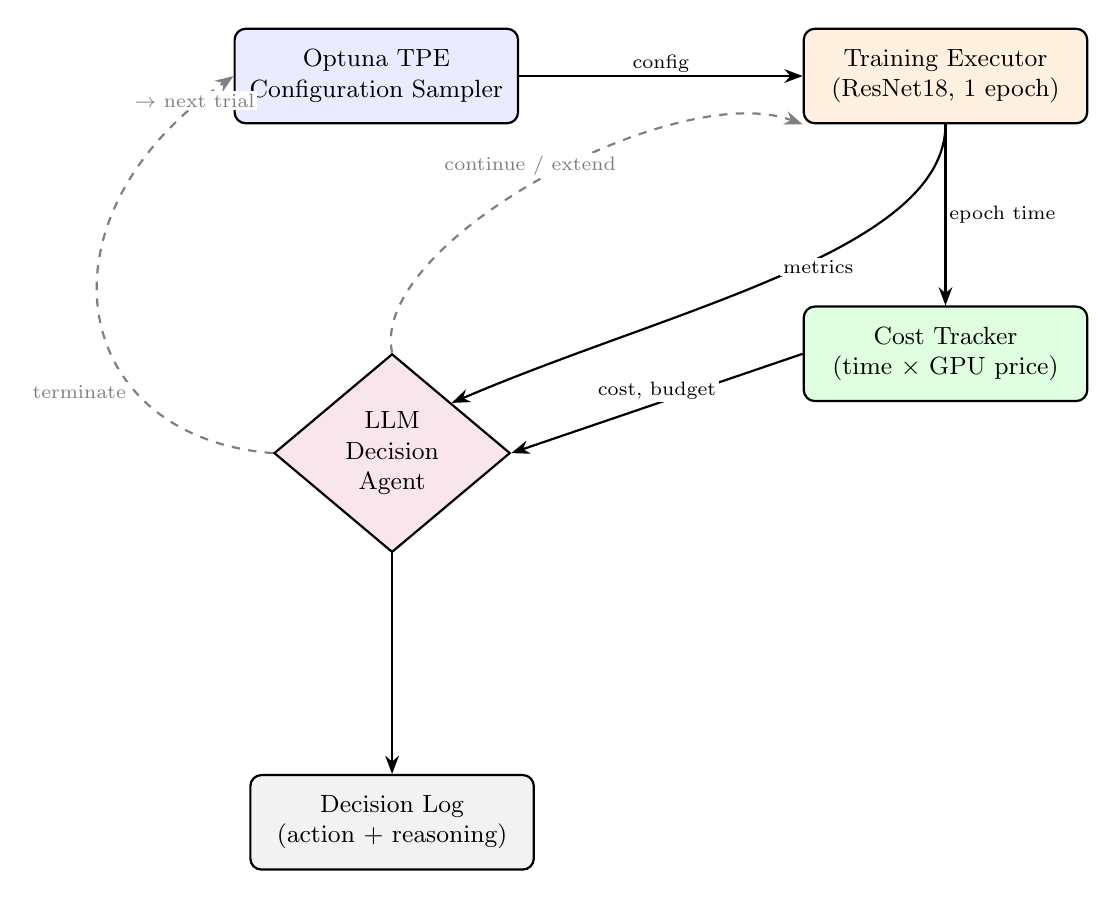
\begin{tikzpicture}[
    node distance=2.3cm and 3.6cm,
    box/.style={rectangle, rounded corners, draw=black, thick, minimum width=3.6cm, minimum height=1.2cm, align=center, font=\small, fill=white},
    decision/.style={diamond, draw=black, thick, minimum width=3.0cm, minimum height=2.2cm, align=center, font=\small, inner sep=2pt, fill=white},
    fwd/.style={-Stealth, thick, black},
    fb/.style={-Stealth, thick, black!50, dashed},
    lbl/.style={font=\scriptsize, fill=white, inner sep=1pt}
]

% ---- main nodes ----
\node[box, fill=blue!8]    (sampler) {Optuna TPE\\Configuration Sampler};
\node[box, fill=orange!12, right=of sampler] (train) {Training Executor\\(ResNet18, 1 epoch)};
\node[box, fill=green!12,  below=of train]   (cost)  {Cost Tracker\\(time $\times$ GPU price)};
\node[decision, fill=purple!10, below=2.9cm of sampler, xshift=0.2cm] (agent) {LLM\\Decision\\Agent};
\node[box, fill=gray!10, below=2.8cm of agent] (log) {Decision Log\\(action + reasoning)};

% ---- forward data flow (solid) ----
\draw[fwd] (sampler) -- (train) node[lbl, midway, above] {config};
\draw[fwd] (train) -- (cost) node[lbl, midway, right] {epoch time};
\draw[fwd] (cost.west) -- (agent.east) node[lbl, midway, above] {cost, budget};
\draw[fwd] (agent) -- (log) node[lbl, midway, right] {};
\draw[fwd] (train.south) .. controls +(0,-1.6) and +(2.8,1.2) .. (agent.north east)
    node[lbl, pos=0.5, above right=-1pt] {metrics};

% ---- feedback / control loops (dashed), kept clear of the forward flow ----
\draw[fb] (agent.north) .. controls +(-0.3,1.4) and +(-1.6,0.6) .. (train.south west)
    node[lbl, pos=0.5, above, xshift=-4pt] {continue / extend};
\draw[fb] (agent.west) .. controls +(-2.6,0.2) and +(-2.6,-1.8) .. (sampler.west)
    node[lbl, pos=0.3, left, xshift=-2pt] {terminate}
    node[lbl, pos=0.92, above, xshift=2pt] {$\rightarrow$ next trial};

\end{tikzpicture}
\caption{System architecture. The Optuna sampler proposes a configuration, which is trained one epoch at a time by the training executor. Solid arrows show the forward data flow: configuration, epoch time, live training metrics, and cost/budget state all feed into the LLM decision agent. Dashed arrows show the agent's control loop: it either signals the training executor to continue/extend the current trial, or terminates it and hands control back to the sampler for the next trial. Every decision is written to the decision log together with the agent's natural-language justification.}
\label{fig:architecture}
\end{figure}

\subsection{Problem Formulation}

Let $\mathcal{X}$ denote the hyperparameter search space, and let $x \in \mathcal{X}$ denote a candidate configuration (learning rate, batch size, optimizer, etc.). For a given trial $x$, let $a_t(x)$ denote the validation accuracy at epoch $t$, and let $c_t(x)$ denote the cumulative simulated dollar cost incurred by trial $x$ up to and including epoch $t$. Let $B$ denote the total budget allocated to the entire HPO run, and let $a^{*}$ denote the target validation accuracy the search aims to reach.

The conventional HPO objective, used by accuracy-only methods such as plain TPE search, is
\begin{equation}
x^{*} = \arg\max_{x \in \mathcal{X}} \; a_{T}(x),
\label{eq:conventional}
\end{equation}
where $T$ is a fixed, predetermined number of training epochs per trial, and cost does not appear anywhere in the objective. In contrast, the cost-aware objective proposed in this work is
\begin{equation}
x^{*} = \arg\min_{x \in \mathcal{X}} \; c_{\tau(x)}(x) \quad \text{subject to} \quad a_{\tau(x)}(x) \geq a^{*},
\label{eq:proposed}
\end{equation}
where $\tau(x)$ is the \emph{agent-determined stopping epoch} for trial $x$ --- a variable epoch count decided dynamically by the LLM agent, rather than a fixed constant $T$. The overall search terminates either when some trial satisfies $a_{\tau(x)}(x) \geq a^{*}$, or when the cumulative cost across all trials exhausts the total budget $B$:
\begin{equation}
\sum_{x \in \mathcal{X}_{\text{tried}}} c_{\tau(x)}(x) \; \leq \; B.
\label{eq:budget_constraint}
\end{equation}

\subsection{Cost Estimation Model}

Because experiments are run on free-tier compute (Google Colab) rather than directly billed cloud infrastructure, cost is estimated rather than metered. Wall-clock training time is measured directly, and converted to a simulated dollar cost using a published, on-demand GPU pricing rate. Formally, for epoch $t$ of trial $x$ with measured wall-clock duration $\Delta t_{t}(x)$ (in hours),
\begin{equation}
c_t(x) = c_{t-1}(x) + \Delta t_t(x) \cdot P_{\text{GPU}},
\label{eq:cost_epoch}
\end{equation}
where $P_{\text{GPU}}$ is the assumed hourly GPU rate (e.g., $P_{\text{GPU}} = \$0.526/\text{hr}$ for an AWS \texttt{g4dn.xlarge} instance with a T4 GPU, held constant across all trials for comparability), and $c_0(x) = 0$. The remaining budget available to the search at any point is
\begin{equation}
R = B - \sum_{x' \in \mathcal{X}_{\text{tried so far}}} c_{\tau(x')}(x'),
\label{eq:remaining_budget}
\end{equation}
and $R$ is one of the quantities passed to the LLM agent at every decision point, so that its termination judgment is made with awareness of how constrained the overall search currently is.

\subsection{Agent Decision Process}

At every epoch $t$ of an active trial $x$, the agent is presented with a structured context vector
\begin{equation}
s_t(x) = \big\langle\, a_t(x),\; \Delta a_t(x),\; a_t^{\text{best}},\; c_t(x),\; R \,\big\rangle,
\label{eq:state_vector}
\end{equation}
where $\Delta a_t(x) = a_t(x) - a_{t-1}(x)$ is the epoch-over-epoch accuracy trend and $a_t^{\text{best}}$ is the best accuracy observed by any trial at the same epoch $t$ so far in the search, used as a relative performance reference. The agent's decision function is
\begin{equation}
d_t(x) = \pi_{\text{LLM}}\big(s_t(x)\big) \in \{\texttt{CONTINUE}, \texttt{EXTEND}, \texttt{KILL}\},
\label{eq:decision_function}
\end{equation}
where $\pi_{\text{LLM}}$ denotes the LLM's mapping from context to decision, implemented via a structured prompt (Table~\ref{tab:prompt}) that additionally requires a natural-language justification $r_t(x)$ to be returned alongside $d_t(x)$. If $d_t(x) = \texttt{KILL}$, then $\tau(x) = t$ and the trial terminates; if $d_t(x) = \texttt{CONTINUE}$ or \texttt{EXTEND}, training proceeds to epoch $t+1$ and the process repeats.

\begin{table}[h]
\centering
\small
\begin{tabular}{p{0.95\linewidth}}
\toprule
\textbf{Prompt template (paraphrased structure)} \\
\midrule
You manage a hyperparameter search trial to minimize cloud cost. \\
Trial config: \{learning rate, batch size, optimizer\} \\
Epoch: $t$ of $T_{\max}$ \quad Validation accuracy: $a_t(x)$ \quad Accuracy trend: $\Delta a_t(x)$ \\
Best trial's accuracy at this epoch: $a_t^{\text{best}}$ \\
Cost spent on this trial: $c_t(x)$ \quad Remaining budget: $R$ \\
Return one of \texttt{CONTINUE} / \texttt{EXTEND} / \texttt{KILL}, with a one-sentence reason. \\
\bottomrule
\end{tabular}
\caption{Structure of the state context supplied to the LLM decision agent at each epoch.}
\label{tab:prompt}
\end{table}

\subsection{Datasets}

\textbf{CIFAR-10.} The primary evaluation dataset is CIFAR-10, a widely used benchmark consisting of 60{,}000 $32\times32$ color images across 10 mutually exclusive classes (airplane, automobile, bird, cat, deer, dog, frog, horse, ship, truck), with 50{,}000 images for training and 10{,}000 for testing, evenly distributed across classes. CIFAR-10 is selected because it is small enough to train quickly on free-tier GPU compute (making the 15--20 trials required per method feasible within the project timeline), while still being large and non-trivial enough that hyperparameter choice materially affects convergence speed and final accuracy, which is required for the cost-savings comparison to be meaningful. A fixed train/validation split (e.g., 45{,}000/5{,}000 images from the training set) is used consistently across all trials and both experimental conditions, with the held-out 10{,}000-image test set reserved only for final reporting of the selected configuration's accuracy.

\subsection{Model and Search Space}

The model architecture is ResNet18, adapted for $32\times32$ inputs and a 10-class output layer. The hyperparameter search space $\mathcal{X}$ includes: learning rate ($\eta \in [10^{-4}, 10^{-1}]$, sampled log-uniformly), batch size ($\in \{32, 64, 128\}$), optimizer ($\in \{\text{SGD}, \text{Adam}\}$), and weight decay ($\lambda \in [10^{-5}, 10^{-2}]$, sampled log-uniformly). This space is intentionally kept moderate in size to remain tractable within a two-week project timeline while still providing enough variation in training dynamics for the agent's stopping decisions to be meaningfully tested.

\subsection{Baselines and Evaluation Metrics}

The proposed agent-guided search is compared against a \textbf{random-search baseline} that samples configurations from the same space $\mathcal{X}$ but trains every configuration to a fixed maximum number of epochs $T_{\max}$ with no early stopping ($\tau(x) = T_{\max}$ for all $x$), representing standard practice with no cost-awareness. Where time permits, a secondary \textbf{Optuna TPE baseline} (also without early stopping) is included to isolate the contribution of the stopping mechanism specifically, independent of the configuration sampling strategy. Both conditions use the identical cost model described in Section~3.3 to ensure a fair, apples-to-apples comparison.

Three metrics are reported for each condition:
\begin{enumerate}
    \item \textbf{Total cost to target}: $\sum_{x \in \mathcal{X}_{\text{tried}}} c_{\tau(x)}(x)$ up to the trial that first reaches $a^{*}$.
    \item \textbf{Trials to target}: the number of trials evaluated before $a^{*}$ is first reached.
    \item \textbf{Final accuracy}: the validation (and held-out test) accuracy of the best configuration found within the budget $B$.
\end{enumerate}
In addition to these quantitative metrics, the natural-language justifications $r_t(x)$ produced by the agent for each \texttt{KILL} decision are logged and reported qualitatively, to assess whether the agent's reasoning is sound, consistent, and auditable --- directly addressing the interpretability contribution described in Section~1.5.

\end{document}
